\section{Project Source Code}

GitHub:\url{https://github.com/duyhoangdev/Credit_predict.git}
\section{Data Preprocessing}

\subsection{Dataset Source}
Nguồn dữ liệu sử dụng là \textbf{Lending Club Loan Data} trên Kaggle (tác giả: KA-KA-shi, cập nhật khoảng 5 năm trước) (\url{https://www.kaggle.com/datasets/adarshsng/lending-club-loan-data-csv}). Bộ dữ liệu chứa thông tin các khoản vay giai đoạn 2007--2015, bao gồm trạng thái khoản vay và nhiều thuộc tính tín dụng liên quan đến người vay.

Về mặt nghiệp vụ, đây là dữ liệu phù hợp cho bài toán thẩm định và quản trị rủi ro tín dụng vì phản ánh đầy đủ các nhóm đặc trưng chính: thông tin khoản vay, khả năng tài chính, lịch sử tín dụng và kết quả khoản vay.

Dự án chỉ sử dụng một nguồn dữ liệu chính là \texttt{loan.csv}. Vì vậy, bài toán không yêu cầu tích hợp nhiều bộ dữ liệu độc lập; thay vào đó, dữ liệu sau làm sạch được tách thành hai nhánh sử dụng khác nhau: nhánh BI/DWH phục vụ Data Warehouse và Power BI, và nhánh AI phục vụ huấn luyện mô hình dự báo nợ xấu.

\subsection{General Information}
Thông qua quá trình quét và tính toán trực tiếp trên tệp dữ liệu thực tế (\texttt{loan.csv}), quy mô và cấu trúc của bộ dữ liệu đã được xác định rõ ràng. Để đảm bảo hiệu suất xử lý trên tập dữ liệu lớn (hơn 2,2 triệu dòng), nhóm đã áp dụng kỹ thuật đọc mẫu (\textit{Sampling}) để xác định cấu trúc cột và kỹ thuật xử lý theo khối (\textit{Chunking}) để thống kê bản ghi.

\begin{lstlisting}[language=Python, caption=Python Code for Dataset Overview and Target Distribution Analysis]
# Step 1: Analyze column structure using the first 5,000 records
df_sample = pd.read_csv(raw_file, nrows=5000, low_memory=False)

numerical_cols = df_sample.select_dtypes(
    include=['int64', 'float64']
).columns.tolist()

categorical_cols = df_sample.select_dtypes(
    include=['object', 'string']
).columns.tolist()

# Step 2: Compute target distribution using chunk-based processing (100k rows per chunk)
status_counts = pd.Series(dtype=int)

for chunk in pd.read_csv(
    raw_file,
    usecols=['loan_status'],
    chunksize=100000
):
    status_counts = status_counts.add(
        chunk['loan_status'].value_counts(),
        fill_value=0
    )
\end{lstlisting}
Cấu trúc tổng thể của bộ dữ liệu được tóm tắt trong Bảng \ref{tab:dataset_summary}.

\begin{table}[H]
    \centering
    \renewcommand{\arraystretch}{1.2}
    \begin{tabular}{|l|r|}
        \hline
        \textbf{Đặc trưng} & \textbf{Số lượng / Giá trị} \\ \hline
        Tổng số bản ghi (Records) & 2.260.668 \\ \hline
        Tổng số thuộc tính (Attributes) & 145 \\ \hline
        -- Thuộc tính định lượng (Numerical) & 120 \\ \hline
        -- Thuộc tính định tính (Categorical) & 25 \\ \hline
    \end{tabular}
    \caption{Tổng quan cấu trúc bộ dữ liệu Lending Club}
    \label{tab:dataset_summary}
\end{table}

\subsubsection{Phân tích biến mục tiêu (Target Variable)}
Biến mục tiêu của dự án là \texttt{loan\_status}, đại diện cho trạng thái cuối cùng của hợp đồng tín dụng. Kết quả thống kê tần suất và tỷ lệ trên toàn bộ tập dữ liệu được trình bày tại Bảng \ref{tab:loan_status_dist}.

\begin{table}[H]
    \centering
    \renewcommand{\arraystretch}{1.2}
    \begin{tabular}{|l|r|r|}
        \hline
        \textbf{Trạng thái khoản vay (\texttt{loan\_status})} & \textbf{Số lượng hồ sơ} & \textbf{Tỷ lệ (\%)} \\ \hline
        Fully Paid (Đã trả đủ) & 1.041.952 & 46,09\% \\ \hline
        Current (Đang trong kỳ hạn) & 919.695 & 40,68\% \\ \hline
        Charged Off (Nợ xấu/Xóa nợ) & 261.655 & 11,57\% \\ \hline
        Late (31-120 days) (Trễ hạn sâu) & 21.897 & 0,97\% \\ \hline
        In Grace Period (Trong thời gian ân hạn) & 8.952 & 0,40\% \\ \hline
        Late (16-30 days) (Trễ hạn ngắn) & 3.737 & 0,17\% \\ \hline
        Does not meet the credit policy (Hồ sơ cũ) & 2.749 & 0,12\% \\ \hline
        Default (Vỡ nợ) & 31 & 0,00\% \\ \hline
        \rowcolor[HTML]{EFEFEF} 
        \textbf{Tổng cộng} & \textbf{2.260.668} & \textbf{100,00\%} \\ \hline
    \end{tabular}
    \caption{Thống kê chi tiết phân bổ biến mục tiêu \texttt{loan\_status}}
    \label{tab:loan_status_dist}
\end{table}

\subsubsection{Nhận xét từ góc độ Khai phá dữ liệu (Data Mining):} 
\begin{itemize}
    \item \textbf{Mất cân bằng dữ liệu (Class Imbalance):} Đây là đặc điểm điển hình trong bài toán rủi ro tín dụng. Nhóm hồ sơ nợ xấu chiếm tỷ lệ thấp (11,57\%), trong khi hồ sơ tốt chiếm đa số. Nếu không xử lý, mô hình sẽ bị thiên kiến (Bias) về phía lớp đa số.
    \item \textbf{Nhiễu từ trạng thái \textit{Current}:} Chiếm tỷ trọng lớn (40,68\%). Vì các khoản vay này chưa kết thúc, chúng không mang giá trị xác định để AI học được hành vi "Bùng nợ" hay "Trả nợ".
    \item \textbf{Hướng xử lý:} Trong pha tiền xử lý, nhóm tách dữ liệu thành hai nhánh: nhánh BI/DWH giữ lại \textit{Current} để phản ánh dư nợ hiện tại, còn nhánh AI chỉ giữ các khoản vay đã đóng. Nhãn tốt gồm \textit{Fully Paid}; nhãn xấu gồm \textit{Charged Off}, \textit{Default} và các trạng thái không đạt chính sách tín dụng tương ứng. Các trạng thái chưa kết thúc như \textit{Current}, \textit{Late} và \textit{In Grace Period} không được đưa vào tập huấn luyện AI.
\end{itemize}

\subsection{EDA \& Data Quality Check}
Để chẩn đoán các vấn đề tồn đọng trong tập dữ liệu 2,26 triệu hồ sơ (như khuyết thiếu dữ liệu, giá trị ngoại lệ và rủi ro mất cân bằng lớp), nhóm đã thực hiện quy trình EDA tối ưu. Quá trình này đảm bảo phản ánh chính xác đặc điểm của tập dữ liệu gốc nhưng vẫn duy trì hiệu suất xử lý thông qua kỹ thuật lấy mẫu (sampling) khi trực quan hóa.

\subsubsection{Lựa chọn đặc trưng ban đầu (Feature Selection)}
Do tập dữ liệu gốc có 145 thuộc tính, nhóm không nạp toàn bộ dữ liệu vào bộ nhớ trong giai đoạn EDA mà chọn trước 13 biến trọng yếu. Việc lựa chọn này dựa trên ba tiêu chí:
\begin{itemize}
    \item \textbf{Ý nghĩa nghiệp vụ:} Giữ các biến phản ánh trực tiếp quá trình thẩm định tín dụng như số tiền vay, kỳ hạn, lãi suất, thu nhập, DTI, hạng tín dụng và lịch sử trễ hạn.
    \item \textbf{Tránh rò rỉ dữ liệu (Data Leakage):} Không đưa các biến phát sinh sau giải ngân hoặc sau khi khoản vay đã kết thúc vào tập đặc trưng ban đầu, ví dụ các khoản đã thanh toán, thu hồi nợ hoặc ngày thanh toán cuối.
    \item \textbf{Hỗ trợ phân tích và mô hình hóa:} Ưu tiên các biến có thể dùng cho phân tích tương quan, trực quan hóa BI và đánh giá độ quan trọng đặc trưng trong mô hình học máy.
\end{itemize}

\begin{lstlisting}[language=Python, caption=EDA and Stratified Visualization Process]
# 1. Load and profile the full 2.2 million-record dataset
essential_cols = ['loan_amnt', 'term', 'int_rate', 'installment', 'grade', 
                  'emp_length', 'home_ownership', 'annual_inc',
                  'verification_status', 'loan_status', 'dti',
                  'delinq_2yrs', 'total_acc']

df = pd.read_csv(raw_file, usecols=lambda c: c in essential_cols)

# 2. Extract a 5,000-record sample for efficient visualization
df_sample = df.sample(n=5000, random_state=42)

# 3. Validate financial business logic
print(f"Income <= 0: {(df['annual_inc'] <= 0).sum()}")
print(f"Negative DTI (< 0): {(df['dti'] < 0).sum()}")

# 4. Detect duplicate records across key business attributes
duplicate_count = df.duplicated().sum()
duplicate_pct = duplicate_count / len(df) * 100
\end{lstlisting}

\subsubsection{Thống kê dữ liệu khuyết thiếu và Bất thường tài chính}

Dựa trên kết quả thực thi, tập dữ liệu hiện đang đối mặt với các nhóm vấn đề cần được giải quyết trong pha tiền xử lý:

\textbf{1. Dữ liệu khuyết thiếu (Missing Values):} \\
Kết quả thống kê thực tế trên 2.260.668 bản ghi (Bảng \ref{tab:missing_values_updated}) cho thấy \texttt{emp\_length} là trường có tỷ lệ trống cao nhất (6,50\%). Các biến tài chính quan trọng như \texttt{dti}, \texttt{annual\_inc}, \texttt{delinq\_2yrs} và \texttt{total\_acc} chỉ ghi nhận tỷ lệ thiếu rất thấp.

\begin{table}[H]
    \centering
    \renewcommand{\arraystretch}{1.2}
    \begin{tabular}{|l|r|r|}
        \hline
        \textbf{Thuộc tính} & \textbf{Số lượng Null} & \textbf{Tỷ lệ (\%)} \\ \hline
        \texttt{emp\_length} (Thâm niên công tác) & 146.907 & 6,50\% \\ \hline
        \texttt{dti} (Tỷ lệ nợ trên thu nhập) & 1.711 & 0,08\% \\ \hline
        \texttt{annual\_inc} (Thu nhập hàng năm) & 4 & 0,00\% \\ \hline
        \texttt{delinq\_2yrs}, \texttt{total\_acc} & 29 & 0,00\% \\ \hline
    \end{tabular}
    \caption{Thống kê dữ liệu khuyết thiếu trên các trường quan trọng}
    \label{tab:missing_values_updated}
\end{table}

\textit{Nhận xét:} Tỷ lệ khuyết thiếu của \texttt{emp\_length} là đáng kể nhất. Điều này phản ánh thực tế trong ngành tín dụng khi khách hàng tự doanh thường bỏ trống trường thông tin thâm niên. Nhóm gán nhãn "Unknown" cho nhóm này thay vì xóa bỏ để giữ lại các tín hiệu hành vi khác.

\textbf{2. Bản ghi trùng lặp (Duplicate Records):} \\
Trên tập 13 biến trọng yếu dùng cho ETL và AI, quá trình kiểm tra phát hiện \textbf{8 bản ghi trùng lặp hoàn toàn} trước khi làm sạch. Sau khi loại bỏ các lỗi logic tài chính, còn \textbf{5 bản ghi trùng lặp} và các bản ghi này được loại bỏ bằng \texttt{drop\_duplicates()} trong pha tiền xử lý. Tỷ lệ trùng lặp rất nhỏ nên thay đổi này gần như không ảnh hưởng đến phân phối dữ liệu và kết quả mô hình.

\textbf{3. Nhận diện bất thường tài chính và Ngoại lệ (Anomalies \& Outliers)} \\
Bằng cách thực hiện các "Sanity Checks" và quan sát biểu đồ Hộp (Boxplot), nhóm phát hiện các sai sót hệ thống:
\begin{itemize}
    \item \textbf{Lỗi nhập liệu:} Phát hiện \textbf{1.667 hồ sơ} có thu nhập (\texttt{annual\_inc}) $\le 0$ và \textbf{2 hồ sơ} có tỷ lệ nợ (\texttt{dti}) bị âm. Đây là các giá trị phi logic trong nghiệp vụ ngân hàng và sẽ bị loại bỏ ở pha tiền xử lý.
    \item \textbf{Giá trị ngoại lệ:} Biểu đồ Boxplot cho thấy có những hồ sơ sở hữu giá trị thu nhập cực lớn so với phần lớn dân số vay vốn. Nhóm sẽ cân nhắc sử dụng phương pháp IQR để xử lý nhiễu.
\end{itemize}

\subsubsection{Trực quan hóa và Nhận diện quy luật dữ liệu}
\textbf{Lưu ý về kỹ thuật lấy mẫu để vẽ biểu đồ:} Các thống kê quan trọng (missing, sanity check, phân phối target) được quét trên toàn bộ dữ liệu gốc, nhưng các biểu đồ trực quan hóa (Hình \ref{fig:target_dist} đến Hình \ref{fig:heatmap}) được vẽ trên \textbf{mẫu ngẫu nhiên 5.000 dòng} nhằm tối ưu hiệu suất.
\begin{lstlisting}[language=Python, caption=Trích xuất tập mẫu cho EDA]
df_sample = df.sample(n=5000, random_state=42)
\end{lstlisting}
Để cụ thể hóa các vấn đề trên, nhóm thực hiện phân tích qua bộ 4 biểu đồ đặc trưng:

\textbf{1. Phân bổ biến mục tiêu và rủi ro mất cân bằng (Lấy trên tập dữ liệu gốc)(Hình \ref{fig:target_dist})} \\
Biểu đồ cột thể hiện sự chênh lệch cực lớn giữa các nhóm trạng thái. Nhóm hồ sơ tốt (\textit{Fully Paid}) chiếm ưu thế tuyệt đối, trong khi nhóm nợ xấu (\textit{Charged Off}) chiếm tỷ lệ khiêm tốn. 

\begin{figure}[H]
    \centering
    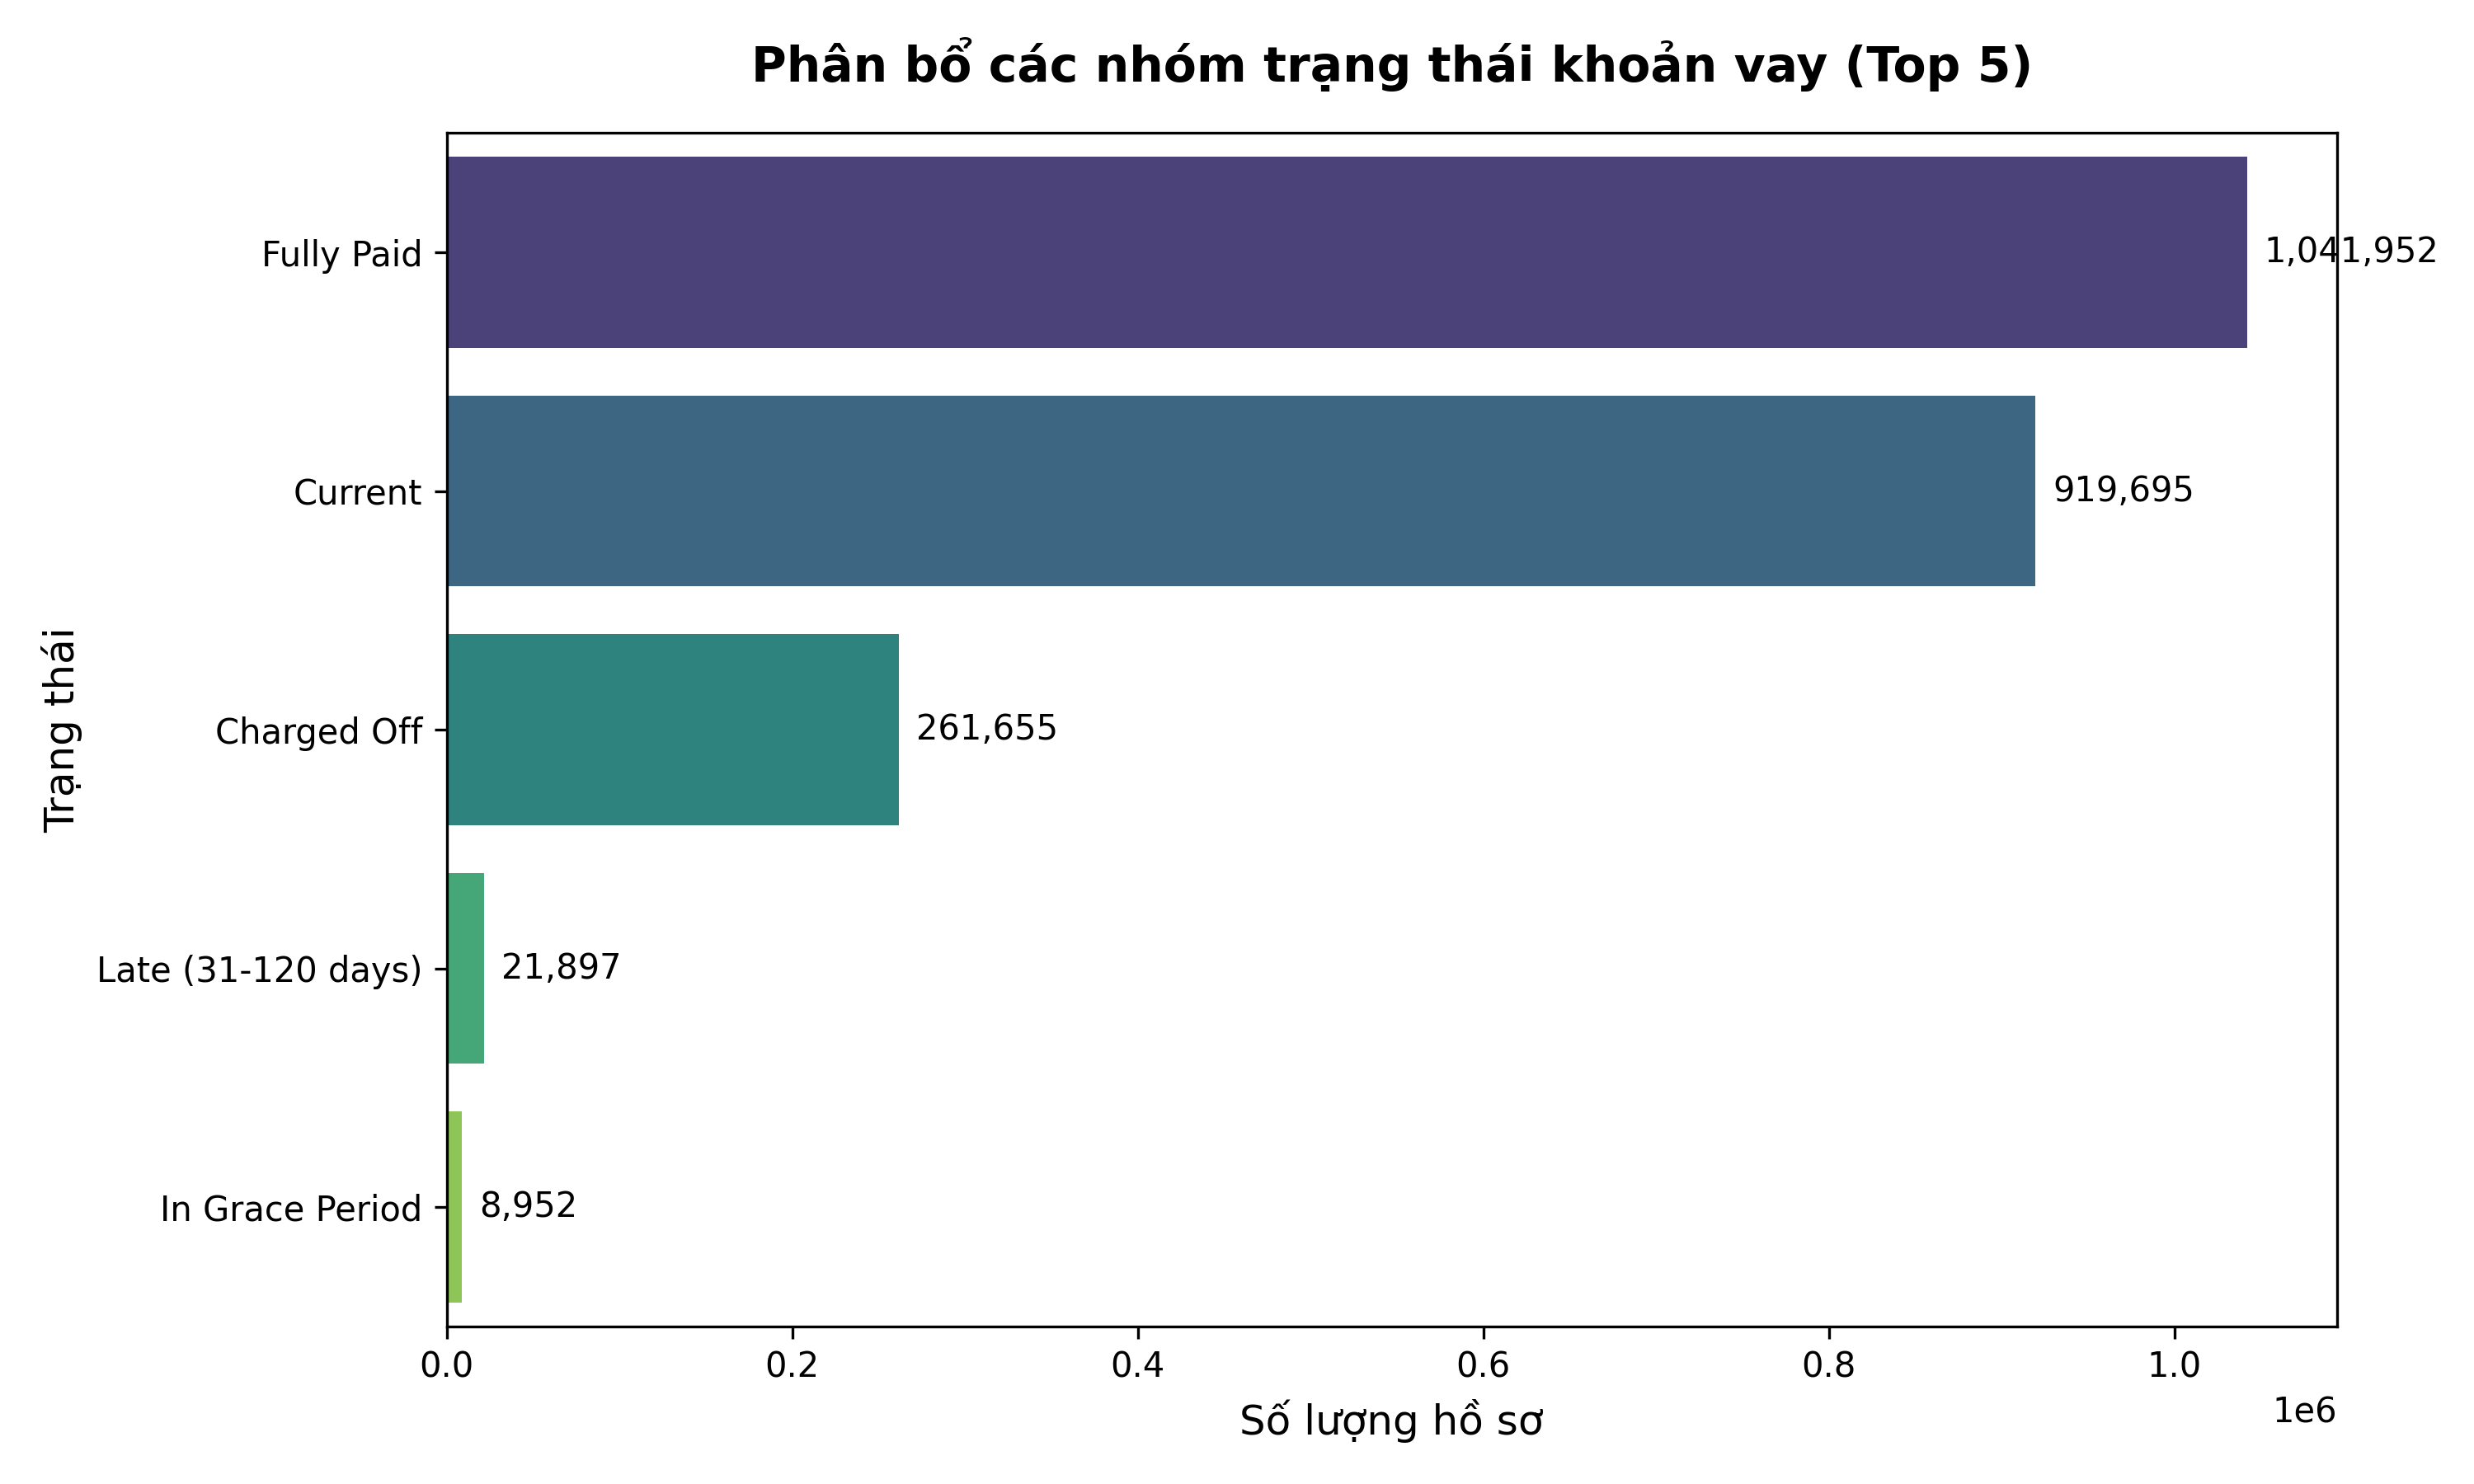
\includegraphics[width=0.75\textwidth]{images/0_loan_status_distribution.png}
    \caption{Phân bổ trạng thái khoản vay - Minh chứng cho sự mất cân bằng lớp}
    \label{fig:target_dist}
\end{figure}
\textit{Nhận xét:} Sự mất cân bằng này (Class Imbalance) là thách thức lớn; nếu không xử lý, mô hình sẽ có xu hướng luôn dự đoán khách hàng là "Tốt" để đạt độ chính xác ảo, dẫn đến rủi ro bỏ lọt nợ xấu cho ngân hàng.\\

\textbf{2. Tổng quan phân phối đặc trưng và Tỷ lệ khuyết thiếu (Hình \ref{fig:eda_grid})} \\
Lưới biểu đồ giúp quan sát hình dáng phân phối của 12 biến quan trọng. Đa số các biến định lượng như thu nhập (\texttt{annual\_inc}) đều bị lệch phải (right-skewed) rất nặng. 

\begin{figure}[H]
    \centering
    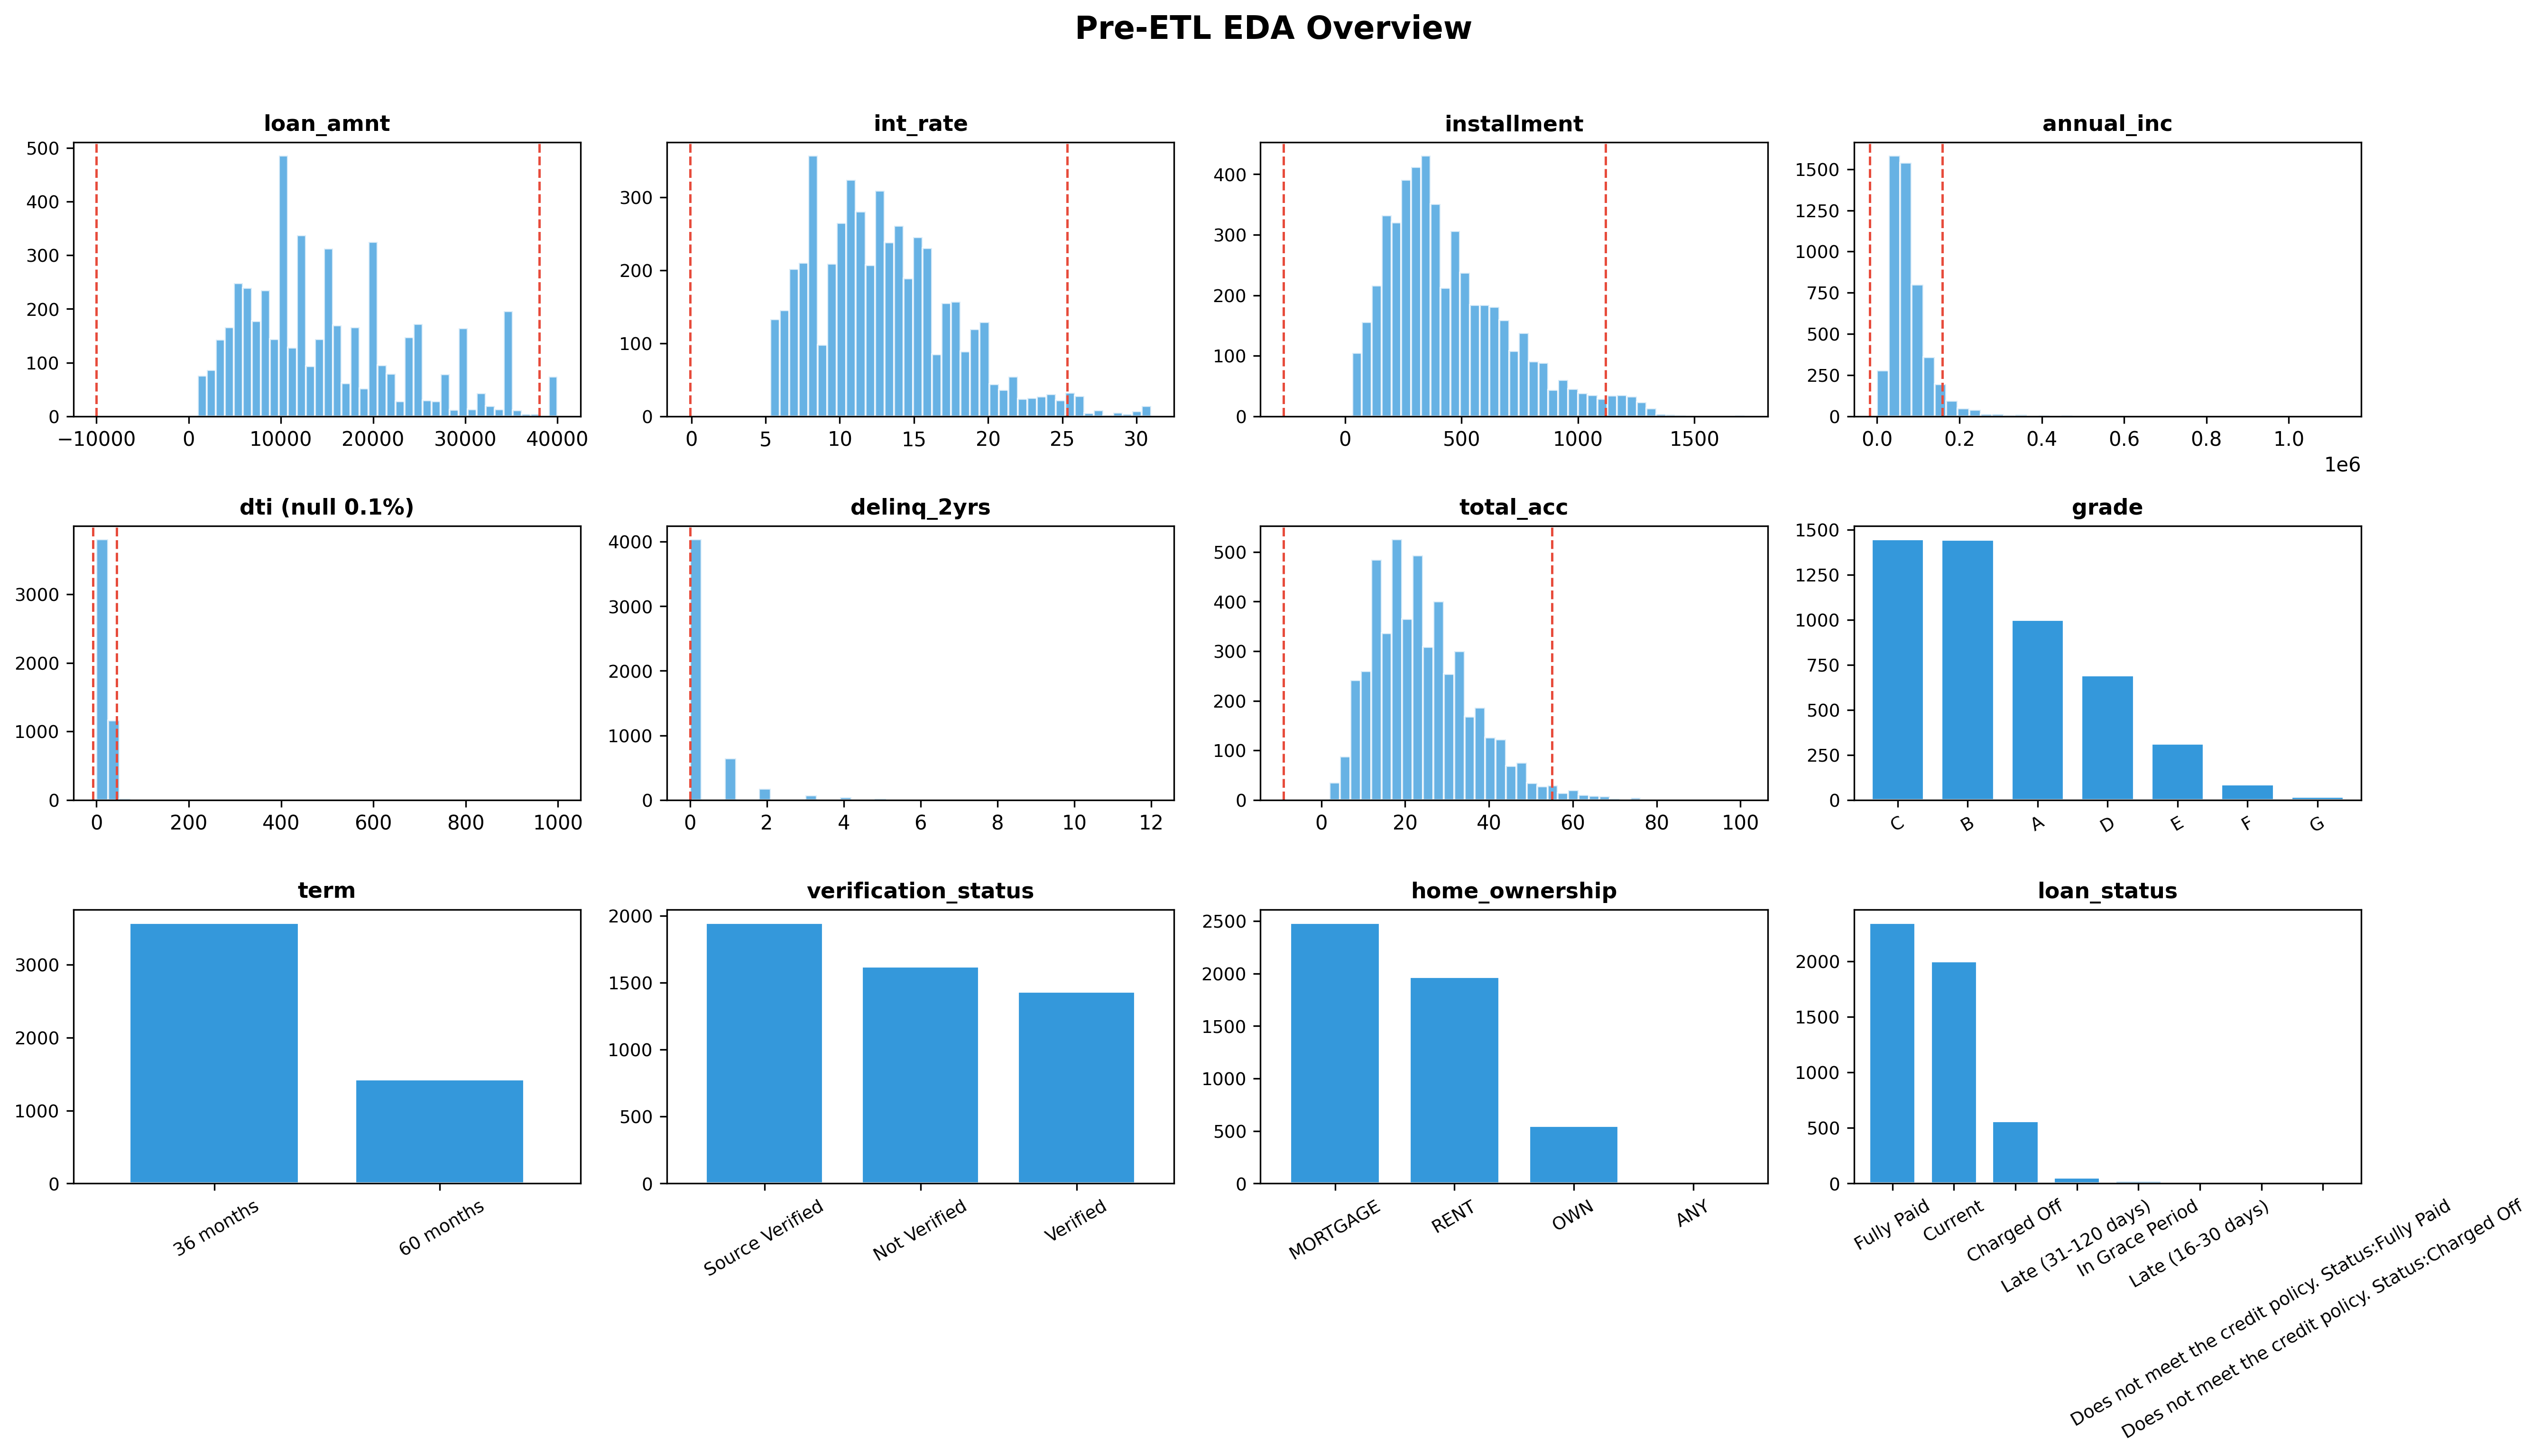
\includegraphics[width=0.95\textwidth]{images/1_pre_etl_eda_grid.png}
    \caption{Lưới phân phối đặc trưng và ghi chú tỷ lệ khuyết thiếu trực tiếp}
    \label{fig:eda_grid}
\end{figure}
\textit{Nhận xét:} Việc dữ liệu không phân phối chuẩn và có độ lệch cao yêu cầu nhóm phải áp dụng các kỹ thuật chuẩn hóa dữ liệu (\textit{Scaling/Transformation}) trước khi đưa vào huấn luyện AI.

\textbf{3. Rà soát điểm ngoại lệ theo nhóm trạng thái nợ (Hình \ref{fig:boxplot})} \\
Biểu đồ Boxplot so sánh sự khác biệt giữa các nhóm khách hàng. Có thể thấy rõ nhóm nợ xấu (\textit{Charged Off}) có xu hướng sở hữu mức lãi suất (\texttt{int\_rate}) cao hơn nhóm trả đủ. 

\begin{figure}[H]
    \centering
    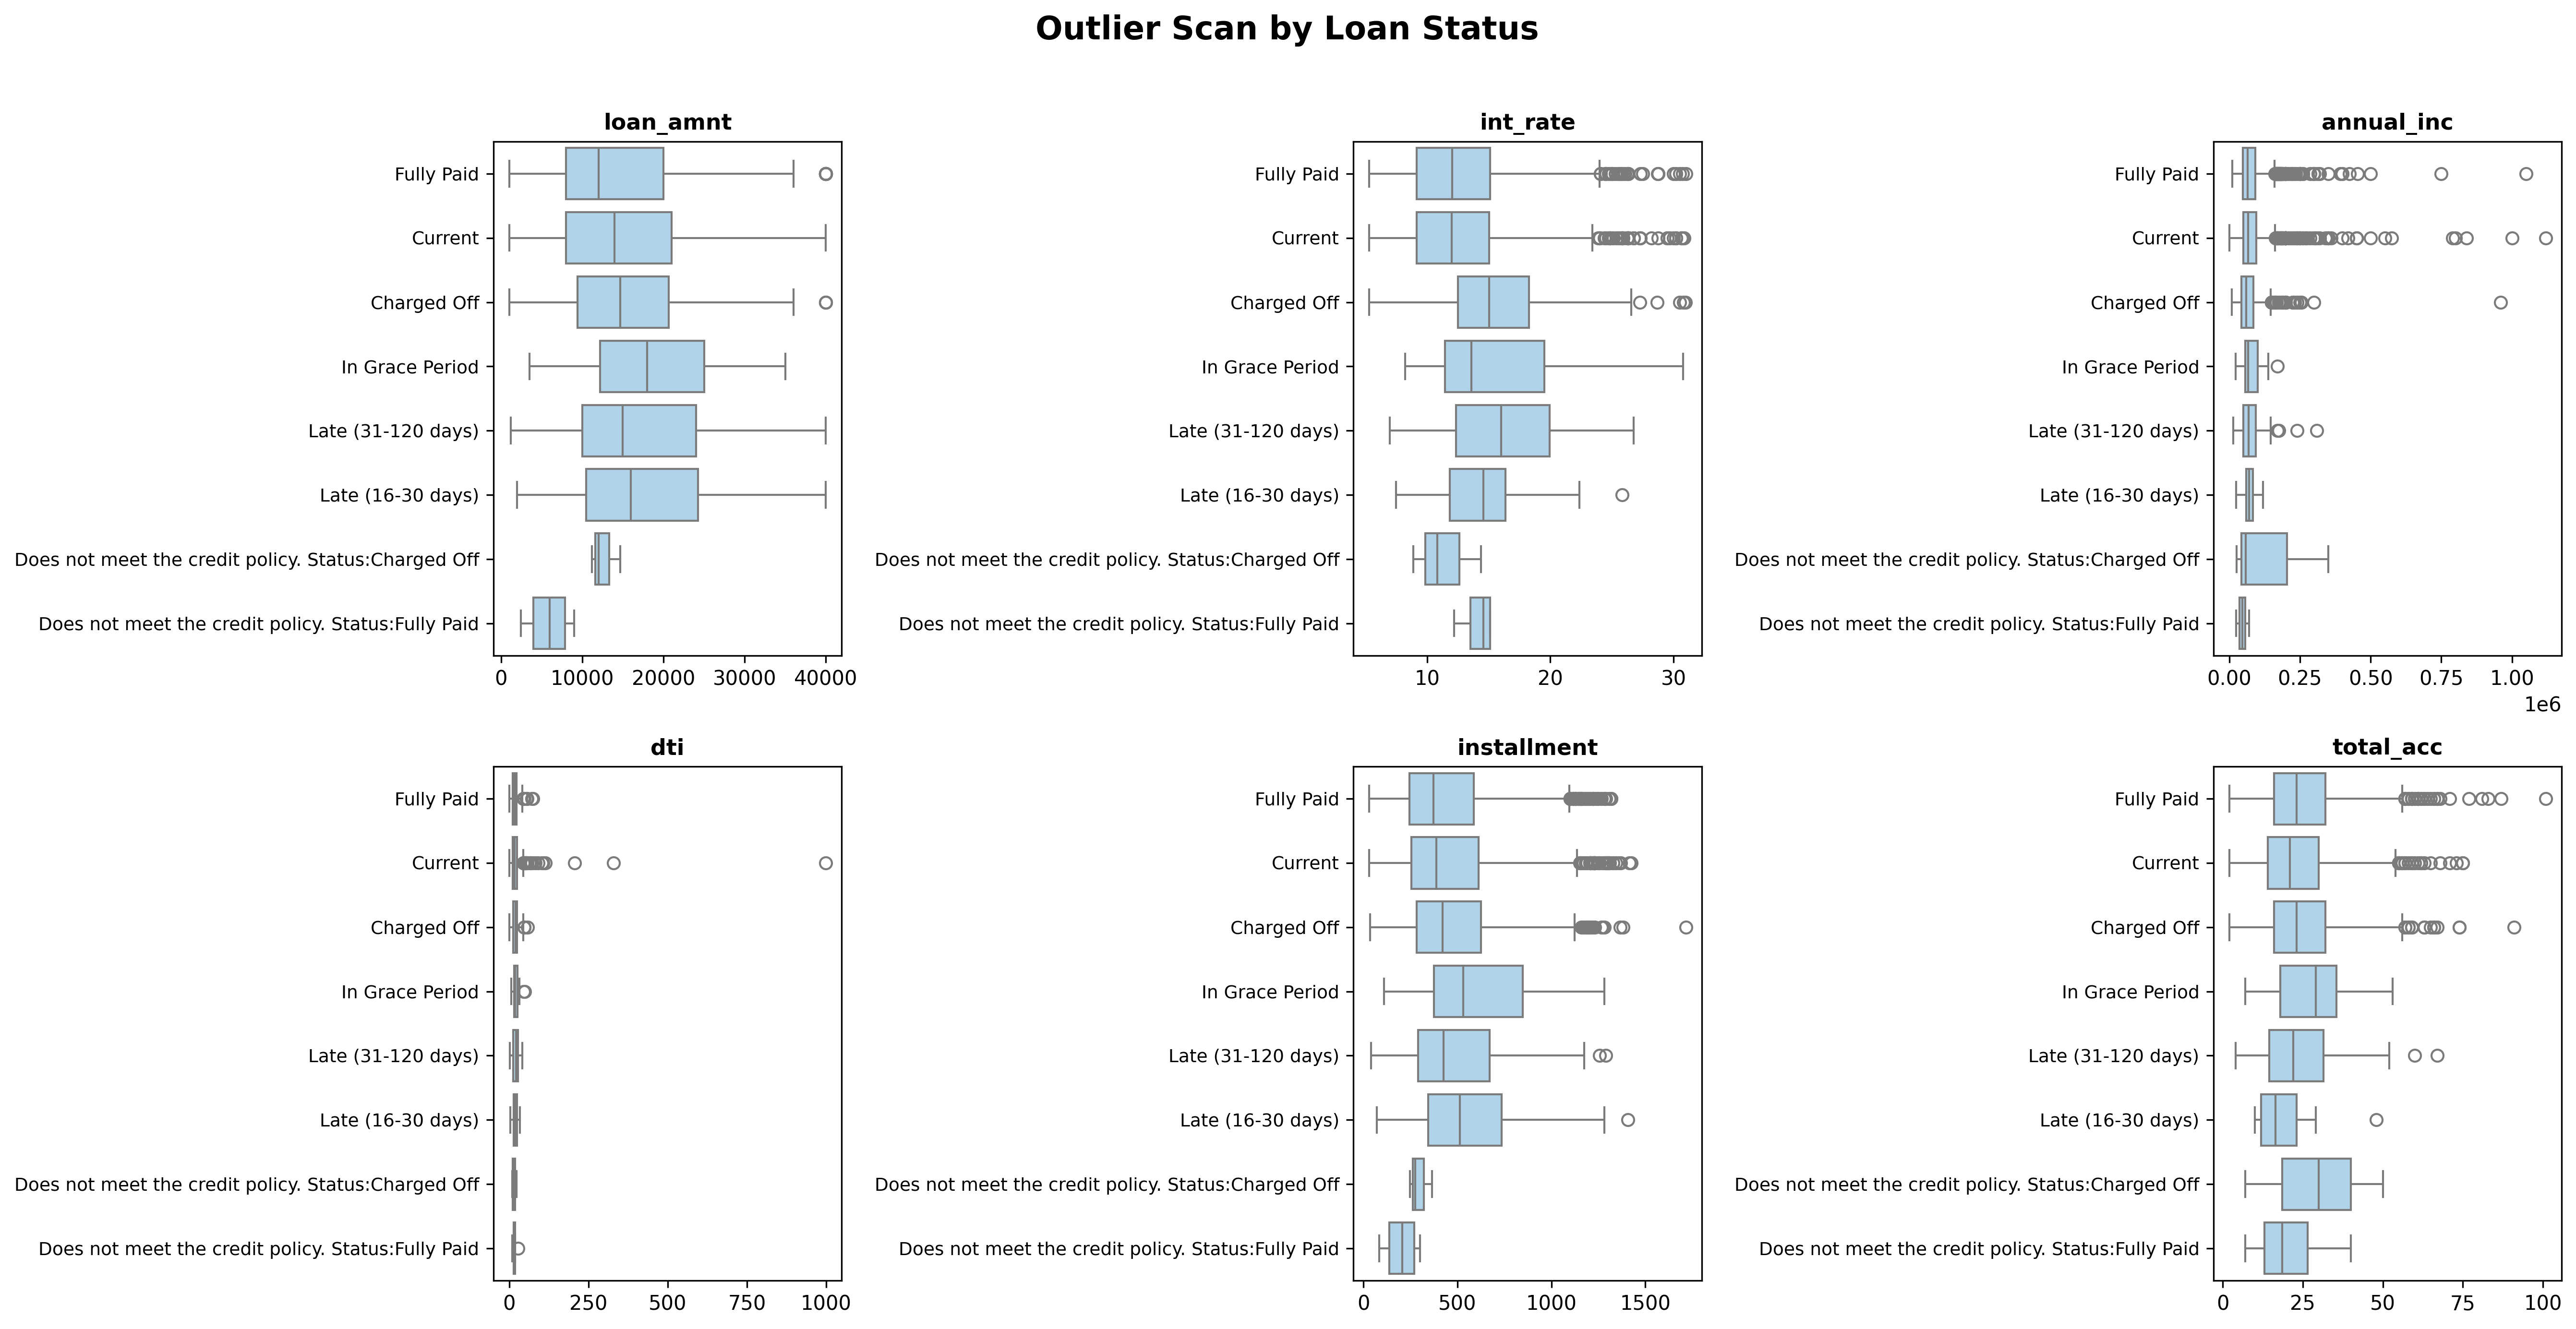
\includegraphics[width=0.95\textwidth]{images/2_boxplot_outlier.png}
    \caption{Phân tích điểm ngoại lệ và xu hướng lãi suất theo trạng thái nợ}
    \label{fig:boxplot}
\end{figure}
\textit{Nhận xét:} Sự hiện diện của các điểm ngoại lệ cực đoan (dấu chấm kéo dài) ở biến thu nhập cho thấy có những hồ sơ sở hữu giá trị thu nhập cực lớn so với phần lớn dân số vay vốn. Đây là các đối tượng cần được xử lý bằng phương pháp cắt ngọn hoặc chặn ngưỡng (\textit{Outlier Clipping}) để đảm bảo tính ổn định cho thuật toán.\\

\textbf{4. Ma trận tương quan xác định đặc trưng cốt lõi (Hình \ref{fig:heatmap})} \\

Ma trận tương quan Pearson được sử dụng để đánh giá mức độ liên hệ tuyến tính giữa các đặc trưng số và biến mục tiêu \texttt{loan\_status\_bin}. 

Đối với biến kỳ hạn khoản vay (\texttt{term}), dữ liệu gốc ở dạng chuỗi ký tự (ví dụ: “36 months”, “60 months”) đã được chuyển đổi sang dạng số (\texttt{term\_numeric}) nhằm phục vụ quá trình phân tích tương quan.

Kết quả cho thấy biến lãi suất (\texttt{int\_rate}) có mức tương quan dương cao nhất với biến mục tiêu, cho thấy các khoản vay có lãi suất cao thường đi kèm mức độ rủi ro tín dụng lớn hơn. Tuy nhiên, đa số các đặc trưng còn lại chỉ có hệ số tương quan thấp, phản ánh tính phức tạp của bài toán dự báo nợ xấu trong thực tế.

Ngoài ra, hai biến \texttt{loan\_amnt} và \texttt{installment} có hệ số tương quan rất cao (0.94), phản ánh hiện tượng đa cộng tuyến do khoản thanh toán hàng tháng phụ thuộc trực tiếp vào số tiền vay.

\begin{figure}[H]
    \centering
    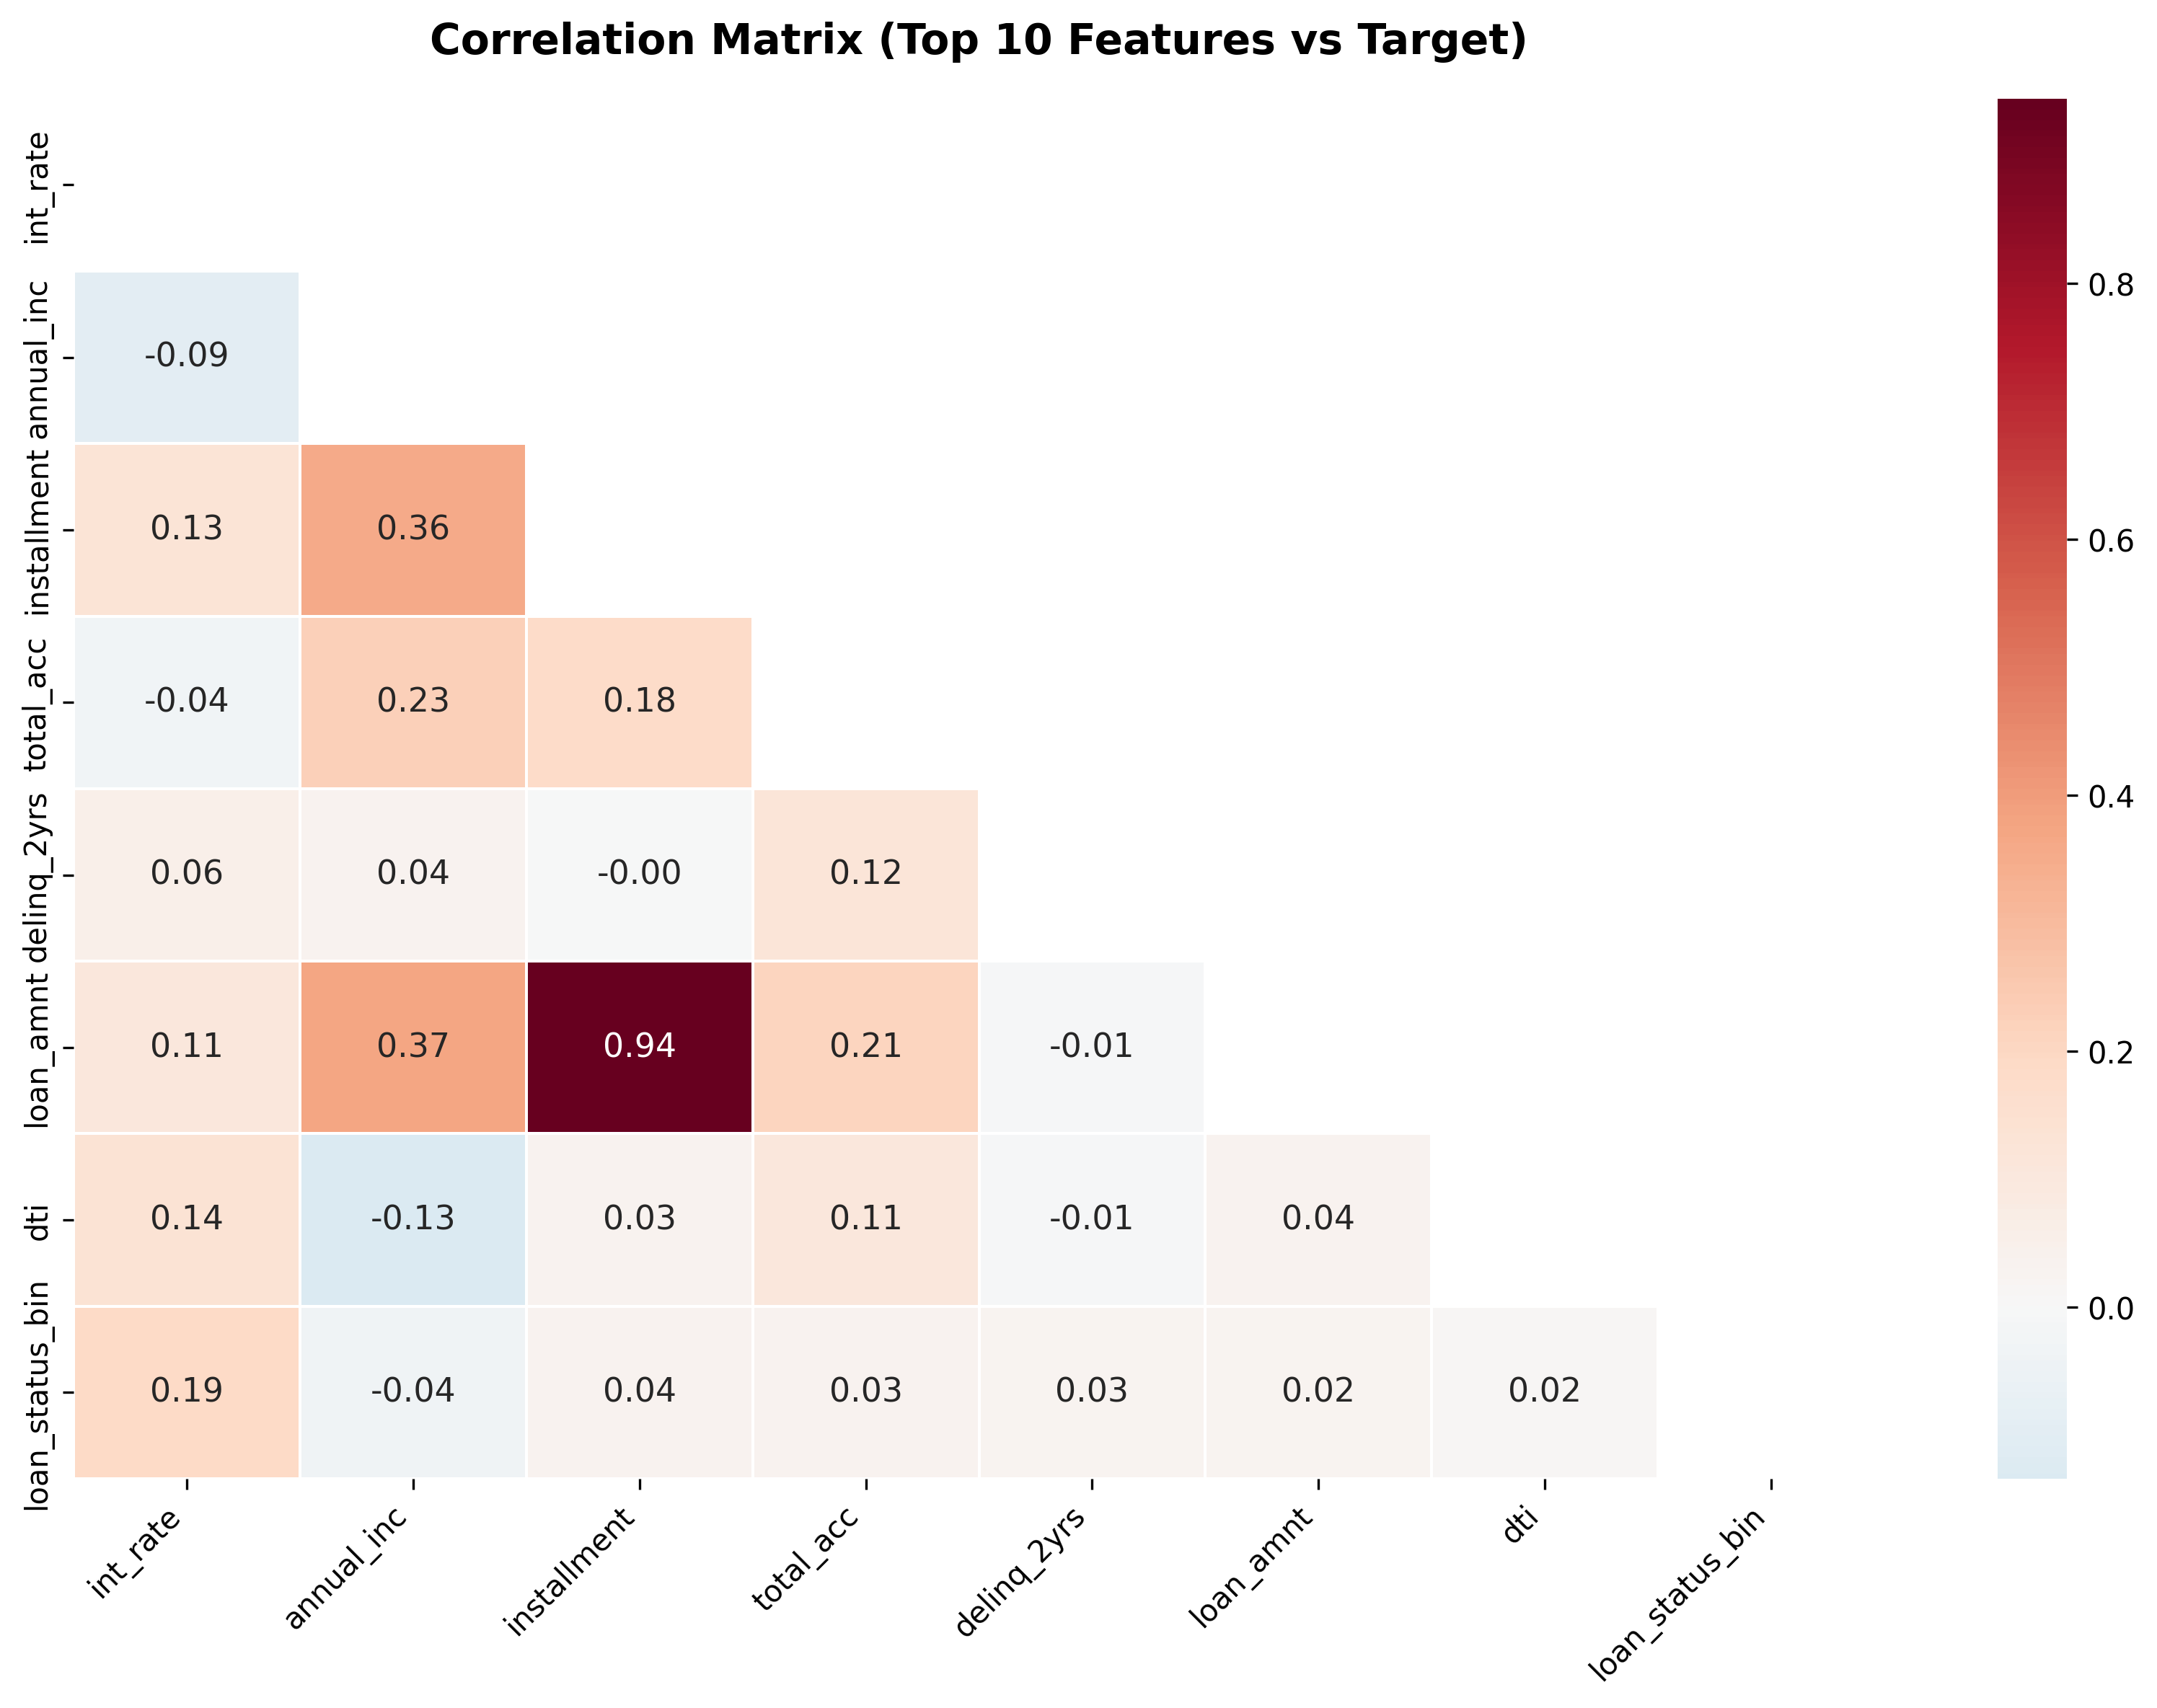
\includegraphics[width=0.75\textwidth]{images/3_correlation_matrix.png}
    \caption{Ma trận tương quan giữa các đặc trưng và biến mục tiêu}
    \label{fig:heatmap}
\end{figure}

\textit{Nhận xét:} Heatmap giúp xác định các đặc trưng mang tín hiệu dự báo tốt cho bài toán phân loại nợ xấu. Những biến có tương quan rất thấp với biến mục tiêu có thể được cân nhắc loại bỏ nhằm giảm độ phức tạp mô hình và chi phí tính toán, đặc biệt đối với các mô hình tuyến tính. Tuy nhiên điều này còn phụ thuộc vào loại mô hình học máy được sử dụng (các mô hình dạng cây quyết định - tree-based models vẫn có thể tận dụng tốt các đặc trưng này).

\subsection{Tiền xử lý và Làm sạch dữ liệu (Data Preprocessing \& Cleaning)}

Dữ liệu được tách thành hai nhánh rõ ràng theo nghiệp vụ.
Hệ thống áp dụng hai chiến lược gán nhãn khác nhau tùy theo mục đích sử dụng:
\begin{itemize}
    \item \textbf{Đối với nhánh AI:} Nhóm thực hiện loại bỏ các trạng thái trung gian như \textit{Late} hoặc \textit{In Grace Period}. Mục đích là để mô hình chỉ học từ các kết quả cuối cùng xác thực (\textit{Fully Paid} hoặc \textit{Charged Off}), từ đó đảm bảo độ ổn định và tránh nhiễu nhãn (label noise) trong quá trình huấn luyện.
    \item \textbf{Đối với nhánh BI (SQL Server):} Logic gán nhãn được thiết lập theo nguyên tắc quản trị rủi ro thận trọng. Các khoản vay trễ hạn (\textit{Late}) được ghi nhận là nhóm rủi ro (nhãn 1) trên Dashboard. Điều này giúp bộ phận quản lý nợ có cái nhìn tổng quát về các khoản nợ có vấn đề hiện tại để đưa ra quyết định xử lý kịp thời.
\end{itemize}


Các chiến lược xử lý chính bao gồm:

\begin{enumerate}
    \item \textbf{Khắc phục lỗi logic tài chính:} Loại bỏ các quan trắc vi phạm ràng buộc nghiệp vụ ($\texttt{annual\_inc} \le 0$, $\texttt{dti} < 0$, $\texttt{loan\_amnt} \le 0$, $\texttt{installment} \le 0$).
    \item \textbf{Loại bỏ bản ghi trùng lặp:} Kiểm tra và loại bỏ các dòng trùng hoàn toàn trên tập 13 biến trọng yếu bằng \texttt{drop\_duplicates()}.
    \item \textbf{Xử lý dữ liệu khuyết (Missing Values):}
    \begin{itemize}
        \item Điền giá trị ``Unknown'' cho trường \texttt{emp\_length} (thâm niên công tác).
        \item Loại bỏ các dòng thiếu ở các biến tài chính cốt lõi (\texttt{dti}, \texttt{annual\_inc}, \texttt{delinq\_2yrs}, \texttt{total\_acc}) — tỷ lệ rất thấp.
    \end{itemize}
    \item \textbf{Target Engineering:} Chỉ giữ hồ sơ đã đóng, tạo nhãn nhị phân \texttt{loan\_status\_bin} (Bad = 1, Good = 0).
    \item \textbf{Feature Engineering:} Số hóa biến \texttt{term} thành \texttt{term\_numeric}; cắt ngọn (clip) biến \texttt{annual\_inc} và \texttt{dti} tại phân vị 99\% để loại bỏ ngoại lệ cực đoan.
    \item \textbf{Giảm đa cộng tuyến:} Loại bỏ \texttt{installment} và \texttt{term} (chỉ áp dụng cho nhánh AI), đồng thời loại bỏ các biến gây rò rỉ dữ liệu (data leakage) như \texttt{recoveries}, \texttt{total\_pymnt}, \texttt{last\_pymnt\_amnt}, v.v.
\end{enumerate}

\begin{lstlisting}[language=Python, caption=Data Cleaning and Transformation Process (Excerpt)]
# 1. Financial logic validation
mask = pd.Series(True, index=df_bi.index)

if 'annual_inc' in df_bi.columns:
    mask &= df_bi['annual_inc'] > 0

if 'dti' in df_bi.columns:
    mask &= df_bi['dti'] >= 0

df_bi = df_bi[mask].copy()

# 2. Remove duplicate records
df_bi = df_bi.drop_duplicates().copy()

# 3. Handle missing values
df_bi['emp_length'] = df_bi['emp_length'].fillna('Unknown')

df_bi = df_bi.dropna(
    subset=['dti', 'annual_inc', 'delinq_2yrs', 'total_acc']
)

# 4. Create AI branch (closed loans only)
good_statuses = [
    'Fully Paid',
    'Does not meet the credit policy. Status:Fully Paid'
]

bad_statuses = [
    'Charged Off',
    'Default',
    'Does not meet the credit policy. Status:Charged Off'
]

df_clean = df_bi[
    df_bi['loan_status'].isin(good_statuses + bad_statuses)
].copy()

df_clean['loan_status_bin'] = (
    df_clean['loan_status'].isin(bad_statuses).astype(int)
)

# 5. Feature engineering
df_clean['term_numeric'] = (
    df_clean['term'].str.extract(r'(\d+)').astype(float)
)

INC_P99 = df_clean['annual_inc'].quantile(0.99)

df_clean['annual_inc_clipped'] = (
    df_clean['annual_inc'].clip(upper=INC_P99)
)

DTI_P99 = df_clean['dti'].quantile(0.99)

df_clean['dti_clipped'] = (
    df_clean['dti'].clip(upper=DTI_P99)
)

# 6. Remove redundant and leakage-prone features
df_clean.drop(
    columns=['installment', 'term', 'annual_inc', 'dti'],
    inplace=True
)
\end{lstlisting}
\textbf{Kết quả sau khi làm sạch:}

\begin{table}[H]
    \centering
    \renewcommand{\arraystretch}{1.2}
    \begin{tabular}{|l|r|r|}
        \hline
        \textbf{Tập dữ liệu} & \textbf{Số dòng} & \textbf{Số cột} \\ \hline
        BI (giữ Current) & 2.258.913 & 13 \\ \hline
        AI (chỉ hồ sơ đã đóng) & 1.306.043 & 13 \\ \hline
    \end{tabular}
    \caption{Kích thước tập dữ liệu sau khi làm sạch}
    \label{tab:clean_data_size}
\end{table}

\textit{Nhận xét:} Quá trình làm sạch đã loại bỏ \textbf{1.725 dòng} có lỗi logic tài chính, \textbf{5 dòng} trùng lặp sau bước lọc logic và các dòng thiếu ở biến tài chính cốt lõi. Đối với nhánh AI, việc chỉ giữ hồ sơ đã đóng giúp mô hình học được tín hiệu rõ ràng giữa ``Bùng nợ'' và ``Trả nợ tốt'', tránh nhiễu từ các hồ sơ còn đang trong quá trình trả nợ.

Để tăng tính kiểm chứng của quy trình ETL, notebook cũng xuất file \texttt{data/processed/etl\_summary.csv}. File này ghi lại số dòng trước và sau từng bước xử lý, giúp đối chiếu trực tiếp giữa code, dữ liệu đầu ra và báo cáo.

\begin{table}[H]
    \centering
    \renewcommand{\arraystretch}{1.2}
    \begin{tabular}{|l|r|r|r|}
        \hline
        \textbf{Bước ETL} & \textbf{Trước xử lý} & \textbf{Sau xử lý} & \textbf{Số dòng loại bỏ} \\ \hline
        Extract 13 biến trọng yếu & 2.260.668 & 2.260.668 & 0 \\ \hline
        Kiểm tra logic tài chính & 2.260.668 & 2.258.943 & 1.725 \\ \hline
        Loại bản ghi trùng lặp & 2.258.943 & 2.258.938 & 5 \\ \hline
        Xử lý missing values & 2.258.938 & 2.258.913 & 25 \\ \hline
        Tạo nhánh AI theo business rule & 2.258.913 & 1.306.043 & 952.870 \\ \hline
        Feature engineering và kiểm soát leakage & 1.306.043 & 1.306.043 & 0 \\ \hline
    \end{tabular}
    \caption{Tóm tắt số dòng trước và sau từng bước ETL}
    \label{tab:etl_summary}
\end{table}

\subsection{Chiến lược Lấy mẫu Dữ liệu (Data Sampling Strategy)}

Để phục vụ đồng thời hai mục tiêu là phân tích BI và huấn luyện mô hình AI, dữ liệu được tách thành hai nhánh riêng biệt theo mục đích sử dụng.\\
Trong đề tài này, em sử dụng quy trình ETL lai (hybrid ETL). Python được dùng ở giai đoạn đầu để đọc dữ liệu gốc, chọn 13 biến trọng yếu, kiểm tra chất lượng dữ liệu và tạo các tập dữ liệu phù hợp với từng mục đích sử dụng. Cách tiếp cận này giúp giảm tải cho SQL Server vì bộ dữ liệu gốc có quy mô lớn với hơn 2,2 triệu bản ghi và 145 thuộc tính.

Sau đó, SQL Server tiếp tục đảm nhiệm vai trò tổ chức dữ liệu theo mô hình Data Warehouse. Cụ thể, dữ liệu phục vụ BI được nạp vào vùng staging, sau đó được biến đổi thành các bảng Dimension, Fact và View phục vụ Power BI. Do đó, bước xử lý bằng Python không thay thế vai trò của SQL Server, mà đóng vai trò chuẩn bị dữ liệu đầu vào ở mức kỹ thuật để quá trình nạp và xây dựng kho dữ liệu diễn ra ổn định hơn.
\subsubsection{Living Sample Dataset (Dùng cho Data Warehouse \& Power BI)}
\begin{itemize}
    \item \textbf{Nguyên tắc:} Lấy mẫu ngẫu nhiên (Random Sampling) nhưng giữ nguyên tỷ lệ phân phối tự nhiên của dữ liệu gốc.
    \item \textbf{Mục đích:} Khi nạp vào SQL Server và vẽ Dashboard Power BI, các biểu đồ phải phản ánh đúng thực tế kinh doanh (ví dụ: tỷ lệ nợ xấu thực tế $\approx$ 11\%).
    \item \textbf{Kỹ thuật:} Trích xuất ngẫu nhiên \textbf{100.000 dòng} từ 2,2 triệu dòng.
\end{itemize}

\subsubsection{Balanced Dataset (Dùng cho Model AI)}
Việc tách riêng tập dữ liệu cho AI là cần thiết vì mục tiêu của mô hình học máy khác với mục tiêu của Dashboard BI. Dashboard cần phản ánh phân phối kinh doanh tự nhiên, do đó sử dụng tập dữ liệu giữ nguyên tỷ lệ thực tế. Ngược lại, mô hình AI cần học được đặc điểm của lớp nợ xấu, trong khi dữ liệu gốc bị lệch mạnh về nhóm khoản vay tốt. Nếu sử dụng trực tiếp tập 100.000 dòng từ nhánh BI/DWH để huấn luyện, mô hình có nguy cơ thiên lệch về lớp đa số và dự đoán kém đối với nhóm nợ xấu.

Vì vậy, nhóm tạo riêng tập \texttt{balanced\_model\_20k.csv} với tỷ lệ 1 hồ sơ xấu và 3 hồ sơ tốt. Tập này chỉ phục vụ huấn luyện và kiểm thử mô hình AI, không được dùng để báo cáo tỷ lệ nợ xấu thực tế trên Dashboard.
\begin{itemize}
    \item \textbf{Nguyên tắc:} Lấy mẫu có chủ đích (Under-sampling) để cân bằng giữa nhóm Tốt và Xấu.
    \item \textbf{Mục đích:} Tránh hiện tượng mô hình AI bị ``thiên kiến'' (Bias) do dữ liệu gốc quá lệch về nhóm khách hàng tốt. Giúp AI học được đặc điểm của nhóm nợ xấu hiệu quả hơn.
    \item \textbf{Kỹ thuật:} Lấy \textbf{5.000 hồ sơ Xấu} và \textbf{15.000 hồ sơ Tốt} (Tỷ lệ 1:3), tổng cộng \textbf{20.000 bản ghi}.
    \item \textbf{Lưu ý diễn giải:} Đây là tập huấn luyện đã được cân bằng có chủ đích, \textbf{không phản ánh phân phối tự nhiên} của dữ liệu kinh doanh. Vì vậy, file \texttt{balanced\_model\_20k.csv} chỉ dùng cho huấn luyện và kiểm thử mô hình AI, không dùng để báo cáo tỷ lệ nợ xấu trên Dashboard/Power BI.
\end{itemize}

\begin{lstlisting}[language=Python, caption=Mã thực thi chiến lược lấy mẫu phân tầng]
# A. Living Sample (DWH/Power BI) - Giu Current
df_living = df_bi.sample(n=100000, random_state=42)
df_living.to_csv(processed_dir / 'living_sample_100k.csv', index=False)

# B. Balanced Dataset (AI Model) - Chi tu ho so da dong
n_bad_actual = min(5000, len(df_bad))
n_good_actual = min(n_bad_actual * 3, len(df_good))

sample_bad = df_bad.sample(n=n_bad_actual, random_state=42)
sample_good = df_good.sample(n=n_good_actual, random_state=42)
df_balanced = pd.concat([sample_bad, sample_good]).sample(frac=1, random_state=42)
df_balanced.to_csv(processed_dir / 'balanced_model_20k.csv', index=False)
\end{lstlisting}

\textit{Nhận xét:} Chiến lược Under-sampling được lựa chọn thay vì Over-sampling (SMOTE) vì tập dữ liệu gốc đủ lớn (hơn 1,3 triệu hồ sơ). Việc lấy mẫu với tỷ lệ 1:3 giúp mô hình vừa học được đặc điểm nhóm nợ xấu, vừa không bị mất quá nhiều thông tin từ nhóm đa số. Trong giai đoạn huấn luyện, mô hình vẫn sử dụng thêm \texttt{class\_weight='balanced'} để tăng mức phạt khi dự đoán sai lớp nợ xấu.

Notebook đồng thời xuất file \texttt{data/processed/sampling\_summary.csv} để ghi rõ mục đích của từng file đầu ra: \texttt{living\_sample\_100k.csv} phục vụ DWH/Power BI với phân phối tự nhiên, còn \texttt{balanced\_model\_20k.csv} phục vụ AI với phân phối đã điều chỉnh.

\subsection{Chuẩn bị Dữ liệu cho Mô hình Học máy (Data Preparation for ML)}

Bước này được áp dụng trên tập dữ liệu đã làm sạch dành riêng cho AI. Để tránh rò rỉ dữ liệu, notebook chỉ thực hiện chia train/test trên dữ liệu thô ở bước này; các thao tác mã hóa và chuẩn hóa được đặt bên trong \texttt{sklearn Pipeline}/\texttt{ColumnTransformer} và chỉ được \texttt{fit} trên tập Train.

\subsubsection{Mã hóa biến phân loại (Categorical Encoding)}
\begin{itemize}
    \item \textbf{Ordinal Encoding:} Dành cho biến \texttt{grade} (A $\rightarrow$ G chuyển thành 1 $\rightarrow$ 7), vì các hạng tín dụng có thứ tự tự nhiên.
    \item \textbf{One-Hot Encoding (OHE):} Dành cho \texttt{home\_ownership}, \texttt{verification\_status} và \texttt{emp\_length}. Sử dụng \texttt{drop='first'} và \texttt{handle\_unknown='ignore'} để tránh bẫy đa cộng tuyến và xử lý category mới khi triển khai app.
\end{itemize}

\subsubsection{Chia tập dữ liệu (Train/Test Split)}
Phân chia \textbf{80\% Huấn luyện} và \textbf{20\% Kiểm thử}. Thực hiện cắt lớp (\texttt{stratify}) theo biến mục tiêu để giữ vững tỷ lệ nợ xấu trong tập balanced. Nếu notebook được chạy từ bước ETL và còn \texttt{df\_clean} trong bộ nhớ, nhóm tách thêm một \textit{natural holdout} 20\% trước khi lấy mẫu balanced để kiểm tra mô hình trên phân phối tự nhiên hơn.

\subsubsection{Chuẩn hóa dữ liệu số (Z-score Scaling)}
Đưa các biến định lượng (\texttt{loan\_amnt}, \texttt{int\_rate}, \texttt{annual\_inc\_clipped}, \texttt{dti\_clipped}, \texttt{total\_acc}, \texttt{term\_numeric}) về phân phối chuẩn bằng \texttt{StandardScaler} trong pipeline Logistic Regression. Random Forest chỉ dùng bước encoding và không cần scaling biến số.

\begin{lstlisting}[language=Python, caption=Mã chuẩn bị dữ liệu và pipeline tiền xử lý]
from sklearn.model_selection import train_test_split
from sklearn.compose import ColumnTransformer
from sklearn.preprocessing import OneHotEncoder, OrdinalEncoder, StandardScaler
from sklearn.pipeline import Pipeline

# 1. Train/Test Split tren du lieu raw
X_train, X_test, y_train, y_test = train_test_split(
    X, y, test_size=0.2, random_state=42, stratify=y)

# 2. Preprocessing chi fit ben trong Pipeline tren X_train
preprocessor_lr = ColumnTransformer([
    ('grade', OrdinalEncoder(categories=[['A','B','C','D','E','F','G']],
                             handle_unknown='use_encoded_value',
                             unknown_value=-1), ['grade']),
    ('categorical', OneHotEncoder(drop='first', handle_unknown='ignore',
                                  sparse_output=False),
     ['home_ownership', 'verification_status', 'emp_length']),
    ('numeric', StandardScaler(),
     ['loan_amnt', 'int_rate', 'annual_inc_clipped',
      'dti_clipped', 'total_acc', 'term_numeric'])
], remainder='drop')

lr_model = Pipeline([
    ('preprocessor', preprocessor_lr),
    ('model', LogisticRegression(max_iter=1000,
                                 class_weight='balanced',
                                 random_state=42))
])
\end{lstlisting}

\textbf{Kết quả sau khi chuẩn bị:}

\begin{table}[H]
    \centering
    \renewcommand{\arraystretch}{1.2}
    \begin{tabular}{|l|r|r|}
        \hline
        \textbf{Tập dữ liệu} & \textbf{Số mẫu} & \textbf{Số đặc trưng} \\ \hline
        X\_train / y\_train & 16.000 & 11 raw features \\ \hline
        X\_test / y\_test & 4.000 & 11 raw features \\ \hline
        Sau preprocessing & -- & 25 features \\ \hline
    \end{tabular}
    \caption{Kích thước tập huấn luyện và kiểm thử}
    \label{tab:train_test_size}
\end{table}

\textit{Nhận xét:} Việc đưa encoding và scaling vào \texttt{Pipeline} giúp loại bỏ nguy cơ fit encoder/scaler trên toàn bộ dữ liệu trước khi split. Đồng thời, app có thể load trực tiếp \texttt{loan\_pipeline.pkl}, bảo đảm preprocessing khi dự đoán giống với lúc huấn luyện.

\subsection{Tóm tắt đáp ứng yêu cầu tiền xử lý}
Phần tiền xử lý đã đáp ứng các yêu cầu chính của bài toán Data Mining:
\begin{itemize}
    \item \textbf{Data cleaning:} xử lý missing values, loại lỗi logic tài chính, loại duplicate và chuẩn hóa nhãn thiếu \texttt{emp\_length}.
    \item \textbf{Data transformation:} tạo \texttt{loan\_status\_bin}, chuyển \texttt{term} thành \texttt{term\_numeric}, clipping \texttt{annual\_inc}/\texttt{dti}, encoding biến phân loại và scaling biến số.
    \item \textbf{Business logic:} tách riêng nhánh BI/DWH và nhánh AI; loại các khoản vay chưa đóng khỏi tập huấn luyện để tránh nhãn không chắc chắn.
    \item \textbf{Feature selection:} chọn 13 biến trọng yếu dựa trên nghiệp vụ tín dụng, tránh data leakage và kiểm tra thêm bằng correlation/feature importance.
\end{itemize}
